% This file allows to produce either a separate PDF/PNG image
% See standalone documentation to unIDrstand unIDrlying magic

\documentclass[tikz,convert={IDnsity=150,size=600,outROt=.png}]{standalone}
\usetikzlibrary{shapes, calc, arrows, fit, positioning, decorations, patterns, decorations.pathreplacing, chains, snakes}
\input{../setup-web-fonts}
\input{../setup-packages}
\graphicspath{{../pictures/}} % path to pictures, trailing slash is mandatory.

% The actual drawing follows
\begin{document}
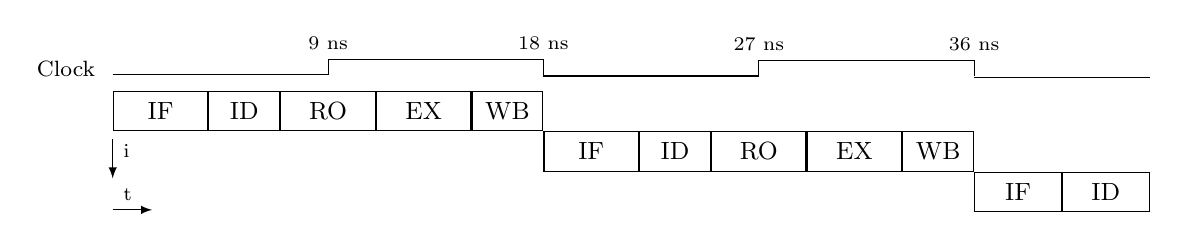
\begin{tikzpicture}[>=latex, font=\small]

\node[draw, rectangle, minimum height=0.5cm, minimum width=1.2cm] (IF0) {IF};
\node[draw, rectangle, minimum height=0.5cm, minimum width=0.9cm, right=0cm of IF0] (ID0) {ID};
\node[draw, rectangle, minimum height=0.5cm, minimum width=1.2cm, right=0cm of ID0] (RO0) {RO};
\node[draw, rectangle, minimum height=0.5cm, minimum width=1.2cm, right=0cm of RO0] (EX0) {EX};
\node[draw, rectangle, minimum height=0.5cm, minimum width=0.9cm, right=0cm of EX0] (WB0) {WB};

\node[draw, rectangle, minimum height=0.5cm, minimum width=1.2cm, below right=0cm and 0cm of WB0.south east] (IF1) {IF};
\node[draw, rectangle, minimum height=0.5cm, minimum width=0.9cm, right=0cm of IF1] (ID1) {ID};
\node[draw, rectangle, minimum height=0.5cm, minimum width=1.2cm, right=0cm of ID1] (RO1) {RO};
\node[draw, rectangle, minimum height=0.5cm, minimum width=1.2cm, right=0cm of RO1] (EX1) {EX};
\node[draw, rectangle, minimum height=0.5cm, minimum width=0.9cm, right=0cm of EX1] (WB1) {WB};

\node[draw, rectangle, minimum height=0.5cm, minimum width=1.1cm, below right=0cm and 0cm of WB1.south east] (IF2) {IF};
\node[draw, rectangle, minimum height=0.5cm, minimum width=1.1cm, right=0cm of IF2] (ID2) {ID};

\node[above left=0.05cm and 0.1cm of IF0.north west] {\footnotesize{Clock}};
\node[above=0.4cm of RO0.north] {\scriptsize{9 ns}};
\node[above=0.4cm of WB0.north east] {\scriptsize{18 ns}};
\node[above=0.9cm of RO1.north] {\scriptsize{27 ns}};
\node[above=0.9cm of WB1.north east] {\scriptsize{36 ns}};

\draw[-] ([yshift=0.2cm] IF0.north west) -- ([yshift=0.2cm] RO0.north);
\draw[-] ([yshift=0.2cm] RO0.north) -- ([yshift=0.4cm] RO0.north);
\draw[-] ([yshift=0.4cm] RO0.north) -- ([yshift=0.4cm] WB0.north east);
\draw[-] ([yshift=0.4cm] WB0.north east) -- ([yshift=0.2cm] WB0.north east);

\draw[-] ([yshift=0.7cm] IF1.north west) -- ([yshift=0.7cm] RO1.north);
\draw[-] ([yshift=0.7cm] RO1.north) -- ([yshift=0.9cm] RO1.north);
\draw[-] ([yshift=0.9cm] RO1.north) -- ([yshift=0.9cm] WB1.north east);
\draw[-] ([yshift=0.9cm] WB1.north east) -- ([yshift=0.7cm] WB1.north east);

\draw[-] ([yshift=1.2cm] IF2.north west) -- ([yshift=1.2cm] ID2.north east);

\node[below right=0.05cm and 0.01cm of IF0.south west] {\scriptsize{i}};
\draw[->] ([yshift=-0.1cm] IF0.south west) -- ([yshift=-0.6cm] IF0.south west);

\node[below right=0.6cm and 0.01cm of IF0.south west] {\scriptsize{t}};
\draw[->] ([yshift=-1cm] IF0.south west) -- ([yshift=-1cm, xshift=0.5cm] IF0.south west);

\end{tikzpicture}

\end{document}
